% !TEX root = ../Dokumentation.tex
\subsection{Fahrbahnerkennung}
\textbf{Funktionsbeschrieb}\\
Die Fahrbahnerkennung soll primär mittels Kamera umgesetzt werden. Dazu werden Bilder aus dem zu Verfügung gestellten Bilderpool entnommen, mit OpenCV in Graustufen umgewandelt und anschliessend einer Kantenanalyse unterzogen. Dazu wird ein eigener Algorithmus verwendet, der jeweils eine Bildzeile als Graph einer Funktion $y = f(x)$ angeschaut, wobei $x$ der Pixelkoordinate der Spalte und $y$ dem Graustufenwert des Pixels entspricht.\\
Anhand der vorhandenen Informationen kann die Fahrbahn und demzufolge während der Fahrt der Korrekturvektor ermittelt werden. Die Korrektur selber soll mittels PID-Regelung realisiert werden, um eine ruhige Fahrt zu erreichen.\\
\textbf{Komponentenbeschrieb}
\begin{figure}[h!]%Position festigen
\centering
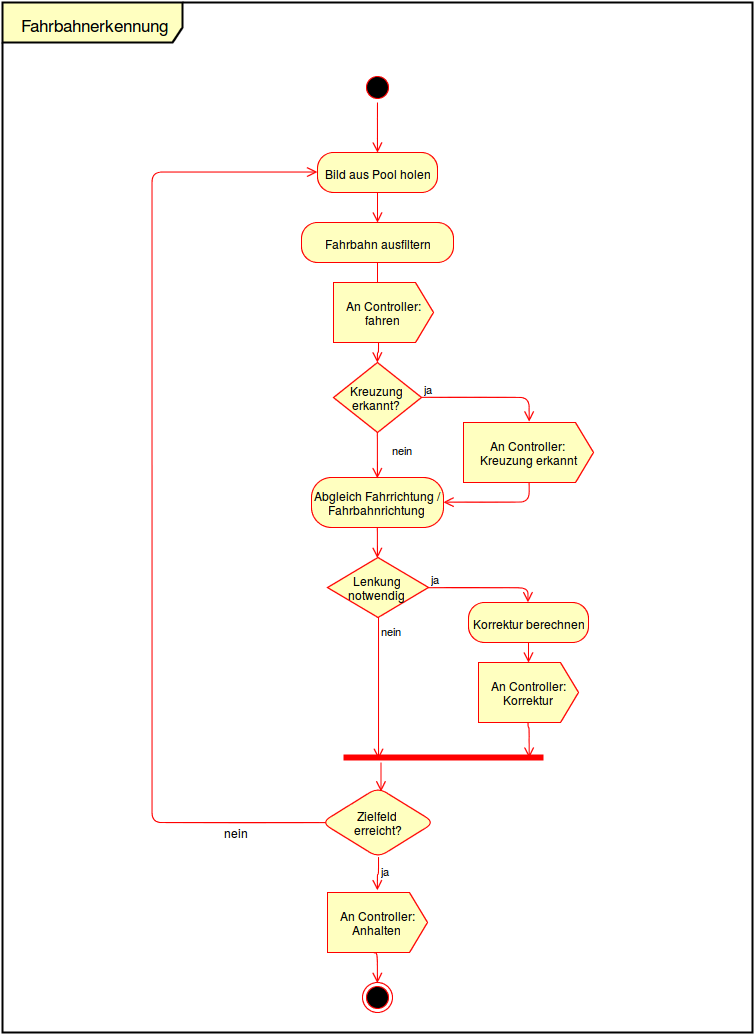
\includegraphics[width=0.6\textwidth]{03_Loesungskonzept/pictures/Fahrbahnerkennung.png}
\caption{Aktivitätendiagramm Fahrbahnerkennung}
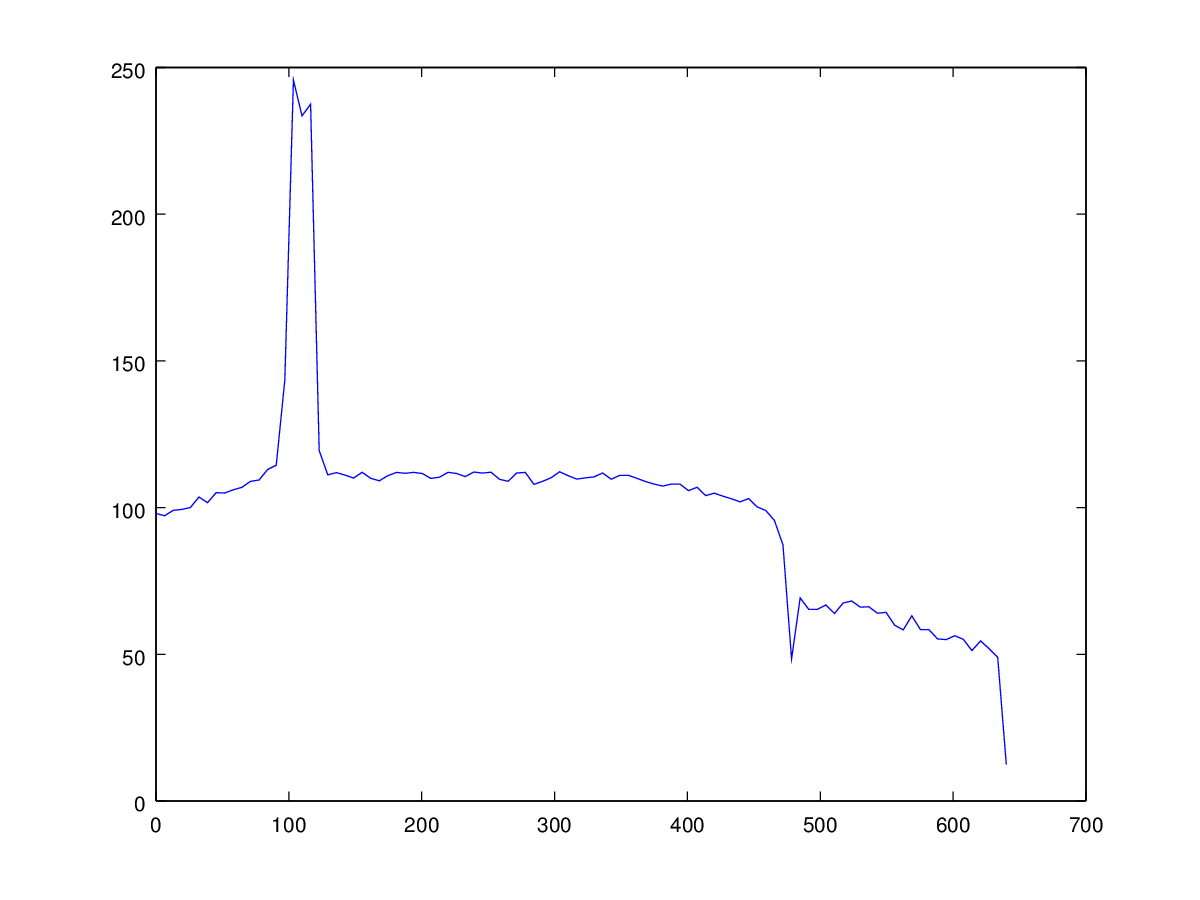
\includegraphics[width=0.6\textwidth]{03_Loesungskonzept/pictures/graphPicture.png}
\caption{Graph der Graustufenwerte einer Bildzeile}
\label{fig:grayscale}
\end{figure}\\
Die Fahrbahnerkennung wird als eigener Thread auf dem Raspberry Pi realisiert und in C++ objektorientiert umgesetzt. Für die Kantenerkennung wird jede Zeile eines Bildes als Funktion angeschaut und falls die Änderungsrate den Filterwert überschreitet eine Kante erkannt (Abbildung). \\
Im Anschluss wird im unteren Bereich des Bildes von innen nach aussen die Fahrbahn gesucht. Dazu werden jeweils in beide Richtungen die ersten Kanten gesucht, über mehrere Punkte fixiert und danach alle übrigen Kanten entfernt.\\
Da die Fahrbahn keine Sprunghaften Änderungen aufweisen kann, wird die Kantendetektierte Matrix von unten nach oben durchgesehen und alle Kanten, die in $x$ - Richtung eine zu grosse Abweichung von der erkannten Fahrbahn aufweisen entfernt, so dass nur noch die rechte und linke Fahrbahnbegrenzung übrig bleibt. Die Mitte zwischen diesen Kanten wird anschliessend in die Zielspur umgewandelt.\\
\textbf{Begründung}\\
Mit der beschriebenen Vorgehensweise kann der Aufwand pro Bild gegenüber OpenCV deutlich reduziert werden, da die Operationen ausschliesslich für die Fahrbahnerkennung erstellt werden. Die Tests haben die Realisierbarkeit dieser Vorgehensweise als machbar und fexibel aufgezeigt.\\
\textbf{Berechnungen}\\
Komplexität des Algorithmus, jedes Bild wird als eine $n\times{m}$ Matrix $M$ betrachtet wobei $n=x$ = Spaltenzahl und $m$ = Zeilenzahl. Die Resultate der Kantenerkennung werden in einer zweiten $n\times{m}$ Matrix $M_1$ gespeichert, welche für die weiteren Berechnungen verwendet wird.
\begin{itemize}
\item Iteration für Kantenerkennung:
\[
n \cdot m \leq n \cdot n \text{ wenn } n\geq m \rightarrow \mathcal{O}(n^2) \text{ mit den Zeugen }C=1 \text{ und } k = m
\]
\item Iteration für Kantenfindung Fahrbahn:
\[
10m \leq 10n  \text{ wenn } n\geq m \rightarrow \mathcal{O}(n) \text{ mit den Zeugen }C=10 \text{ und } k = m
\]
\item Iteration für Fahrbahnausfilterung und das Erzeugen der Sollspur:
\[
n \cdot m \leq n \cdot n \text{ wenn } n\geq m \rightarrow \mathcal{O}(n^2) \text{ mit den Zeugen }C=1 \text{ und } k = m
\]
\item Zusammengezogene Schätzung der Komplexität:
\begin{align*}
2(n^2) + 10n &\leq 2n^2 + 10n^2 \text{ wenn } n\geq 1\\
             &= 12n^2\\
             &\rightarrow \mathcal{O}(n^2) \text{ mit den Zeugen }C=12 \text{ und } k = m
\end{align*}
\end{itemize}
Formeln für die Berechnungen:
\begin{itemize}
\item Kantenfindung $h=$ Grenzwert für die Änderungsrate um eine Kante zu ermitteln und $y_1$ der Wert des Pixels in der Zielmatrix $M_1$:
\[
y = f(x) = \text{ Graustufen des Pixels }0 \leq y \leq 255
\]
$x:=1 \text{ to } n-2 \text{ step } 1$\\ 
$\textbf{if } f(x+2)-f(x) \geq h \textbf{ then } y_1 = 255 \textbf{ else } y_1 = 0$\\
\end{itemize}
\textbf{Testergebnisse}\\